
% thesis.tex (also saved as simple.tex) -- a simple thesis document
% for demonstrating dalthesis.cls class file, or to use as a starting
% document for writing a thesis.
% If you are not familiar with TeX and LaTeX, the first thing that you
% can learn that line comments start with the percent sign (%), so
% these lines are ignored by the system.  Feel free to change them or
% delete them.
\documentclass[12pt]{report}
\newcommand{\mychapter}[2]{
    \setcounter{chapter}{#1}
    \setcounter{section}{0}
    \chapter*{#2}
    \addcontentsline{toc}{chapter}{#2}
    }
\usepackage[utf8]{inputenc}
\usepackage{graphicx}
\usepackage{gensymb}
\usepackage{comment}
\usepackage{amsmath}
\usepackage{caption}
\usepackage{subcaption}
\usepackage{pdfpages}
\usepackage[toc,page]{appendix}
\usepackage{afterpage}

\newcommand\blankpage{%
    \null
    \thispagestyle{empty}%
    \addtocounter{page}{0}%
    \newpage}
\usepackage{hyperref}

\pagenumbering{roman}

\begin{document}


\begin{figure}
 \centering 
 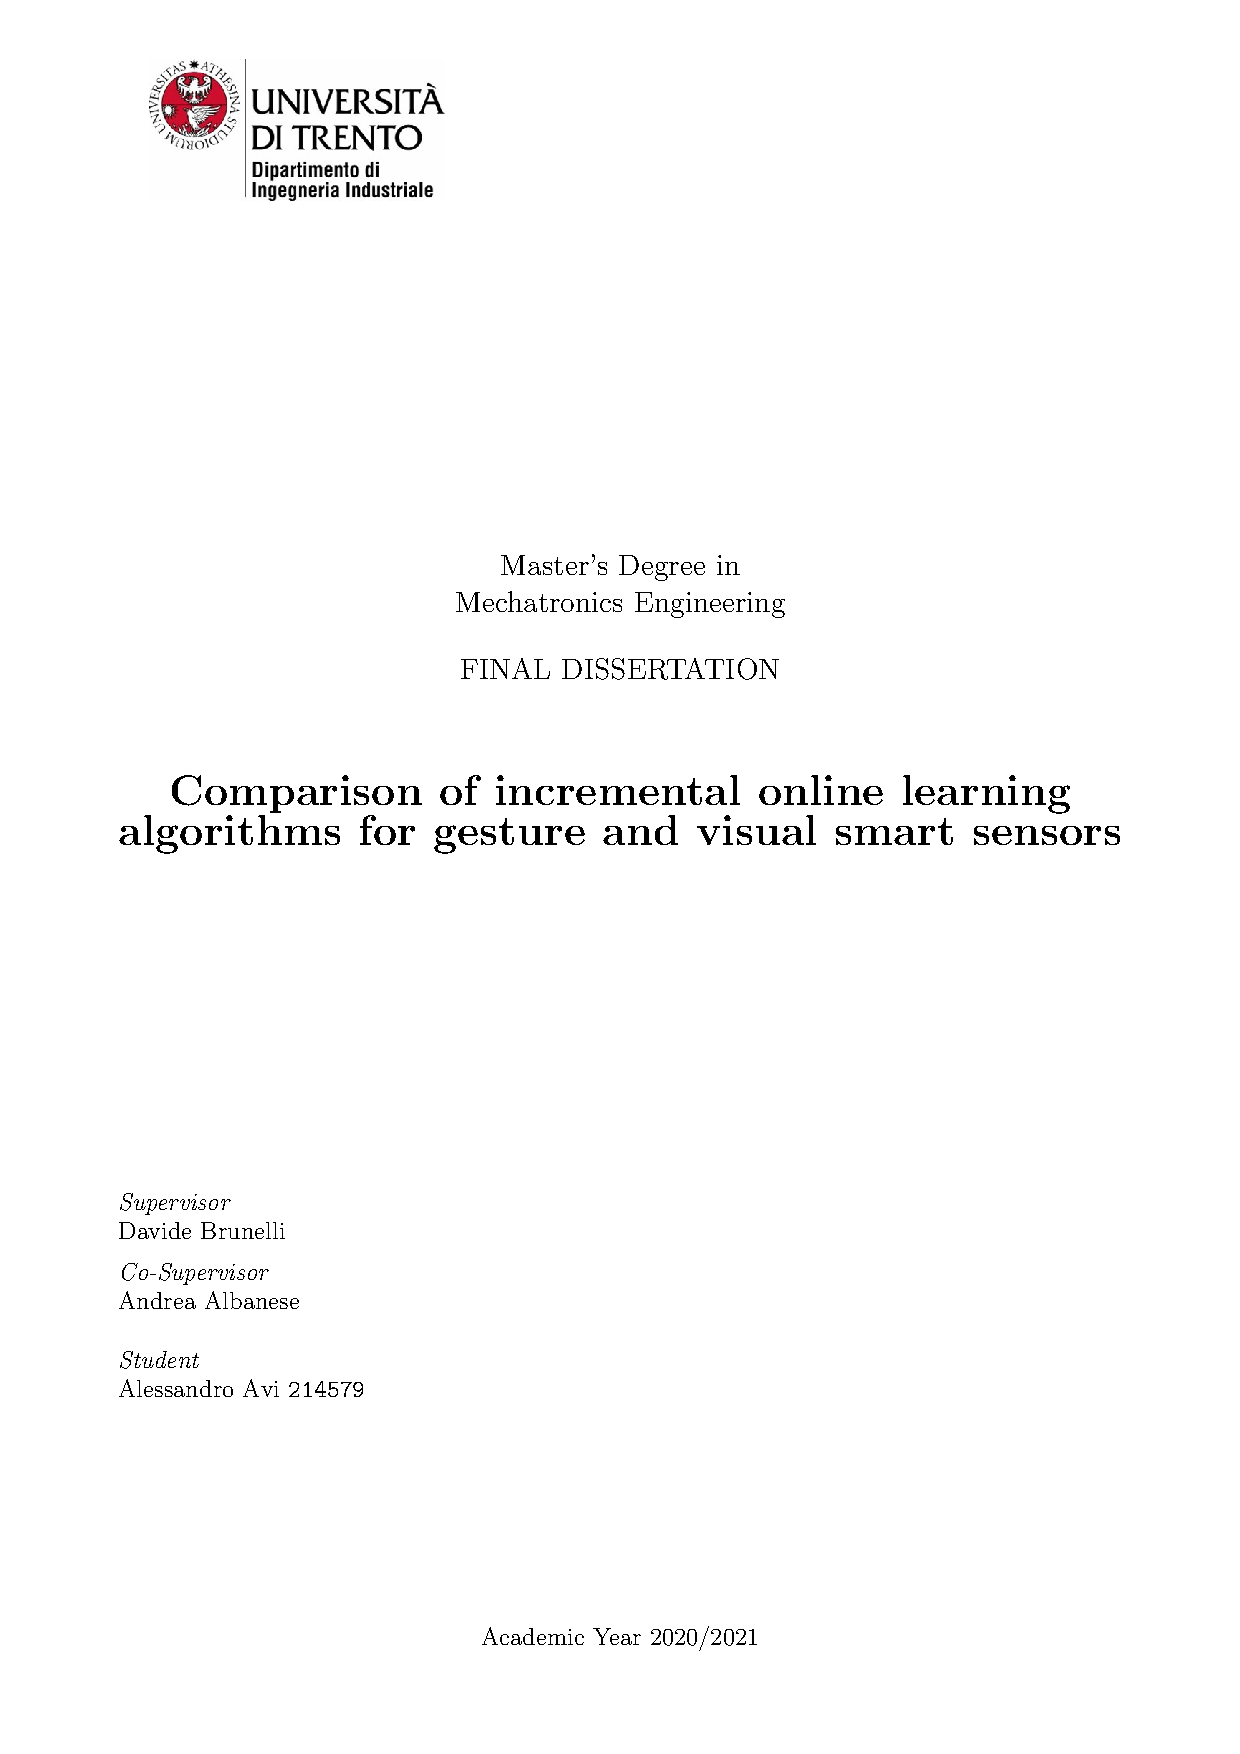
\includepdf[pages=-]{Figures/frontespizio.pdf}
\end{figure}

\afterpage{\blankpage}

\chapter*{}
\vspace*{\fill}
\textit{"Ciao."} 
\begin{flushright}
Mario
\end{flushright}
\vspace*{\fill}

\afterpage{\blankpage}





%\afterpage{\blankpage}
\tableofcontents
%\afterpage{\blankpage}
\listoffigures
\listoftables
\afterpage{\blankpage}



%\mainmatter

\mychapter{0}{Introduction}
\pagenumbering{arabic}

The application of machine learning (ML) on small devices, in a word TinyML, is becoming more and more popular as technologies advances. The usage of this type of technology on micro controllers (MCU) is proving to be more indispensable and helpful in several fields like the industrial applications, agricultural automation, autonomous driving, human-machine interaction. One of the main fields in which TinyML shines and is well suited is the world of Internet of Things (IoT). Here machine learning applied on small devices finds its sweet spot since it can be exploited to revolutionize the basics of IoT networks. The ability of embedded systems to perform high level and smart data elaboration makes it possible for the IoT pipeline to change from cloud computing to edge computing. This transformation comes with great benefits and additional challenges. 
First of all the traffic on IoT networks is drastically reduced. In fact by performing inferences and predictions directly on the edge the raw data gets compressed into smaller sequences that are enriched of information, reducing the quantity of data moving int the IoT networks. This allows to reduce the energy consumption dedicated to the entire system. In fact by redirecting the energy flow from data transmission to ML computation it's possible to decrease the consumption by and order of magnitude \cite{} SERVE UNA REFERENCE. 
Not only edge computing lowers the traffic but also it reduces the computational weight given to the central point of the entire network, the cloud. This results in reduced times of computation and communication between edge and cloud, which if combined with the ability of the MCU to perform autonomous decision, reduces the latency of real time applications improving the overall experience. 
Another benefit is the improved privacy of the network which is a direct consequence of the reduction of data transmitted. Of course by having less data transmitted alsothe possibility to have unwanted interceptions is reduced. At last the usage of ML on small devices allows for better customization of the device itself, which can make the devices better suited for the job. 
Of course the application of such a technology comes with a cost, in this case increased complexity and higher amount of vulnerabilities. It's in fact necessary to set up robust systems that are able to ensure the security of the system (due to the high number of vulnerable nodes) and perform at their best, no matter the limitation of the device. It's known that the main downsides of embedded systems and small MCUs are their limited hardware, mainly small memories and batteries. Still these devices are required to perform at their best even with limited computational power and limited power consumption.\\
Another relevant challenge for the application of ML in the world of IoT comes directly from the environment in which these are deployed. Depending on the specific application it's usually the case that the context in which an IoT device lives is not characterized by static behaviour. Meaning that the phenomenon to be monitored is able to change or evolve over time and so does the data recorded. This can make difficult the usage of the ML models because they lack the ability to adapt to the changing scenarios. In fact typical TinyML applications aim at training the models on powerful devices and later deploy them on the MCU, where only the inference is performed. It's clear how these devices are vulnerable to the context change before mentioned. In today's research three different types of scenarios can be defined: New Instances (NI), when new patterns of already known classes are detected; New Classes (NC), when new families of data are found that are not recognized by the system ; New Instances and Classes (NIC), when the data is composed of both new patterns and new classes.
By training ML models for a specific context and later deployng them in the real world is to be expected a drop in prediction accuracy which would make the application itself non reliable. It's then clear how an application of simple ML on such problems is not the best solution. In order to contrast the issue it's necessary to implement what is called Continual Learning (CL). A machine learning approach that allows ML models to be continually kept up to date
This type of machine learning method uses a real time training based on the data incoming, thus allowing the model itself to change and adapt its weights to better contrast the context drift. An additional feature that can be easily added to CL is the recognition of new and never seen classes, that allows the model to also extend its structure in order to better perform inference on the data and be able to recognize new classes. \\
The implementation of CL in industrial applications is not a new topic in the research world, but its implementation on tiny devices is just starting to become more and more popular. The most common applications see CL in industrial scenarios, mainly for monitoring purposes on heavy machines.
The main contributions of this study concern the application of CL in two interesting application. The objective here is to understand if CL is a feasible solution for TinyML and if its usage is actually effective for the generation of autonomous and self adapting models. In this study several state of the art continual learning algorithms are implemented and tested in two experiments, both concerning the application of ML classification on different types of data. The first application regards the analysis of accelerometer data. In this experiment the user holds the accelerometer sensor in its hand and records a time series of accelerations while drawing letters in the air. The idea is to be able to apply ML in order to classify the input data are recognize the letters written. The model created is initially trained for the recognition of the pattern from the vowels. Later CL is applied to the experiment and the model is exposed to new data representing three new consonants. The aim of the experiment is to let the ML model learn the new patterns by performing a real time training. Even if the experiment proposed is closer to an academic study than a real application it's considered to be a clear example of how a CL model could behave in a similar scenario. A popular application of CL in the research is in fact the monitoring of vibration patterns of heavy industrial machinery. The second application sees the experimentation of CL on a CNN model applied on an OpenMV camera for the recognition of the digits from the MNIST dataset. The idea this time is to initially train the model to recognize only the digits from 0 to 5 and later use the CL framework developed for applying a real time training on the remaining digits. This second experiment could be closer to an application, once again in the industry field, where a camera is used for visual control of defects on products in a production pipeline.  \\
The work done for this study is a good example for showing the capabilities of these tiny devices. It proves that machine learning applied on MCUs is a technology that has huge potential and deserves more attention. It could lead to smarter, more efficient, better performing systems in the fields of IOT and applications in the industrial and agricultural world. 

%accennare catastrophic forgetting



\chapter{Related Works}


\section{Machine learning in general}


\section{Machine Learning on MCU}
% applicazione ml su mcu, risorse limitate, molto importante power comsumption, design del mcu, paralre di possibili applicazioni, paraldre del fatto che si fa solo inference
% parlare del rpuning, binarization, compression del meodello, state of teh art compression MCUNET


TinyML is a fast growing research area that aims at applying ML on limited devices like micro controllers. This technology has found a rapid grow in the last years especially thanks to the potential demonstrated by useful applications. The main fields in which TinyML can be applied are human-computer interactions, industrial applications, ... Fare esempi di paper generici su TinyML

The main challenge of TinyML is for sure the successful application of ML on such resource constrained systems. These are in fact designed to be deployed in difficult to reach places and for running for very long times. This implies that the devices should be battery powere or equipped with energy havresting hardware and their power consumption should be limited and optimized. Other limitations concern the limited computational power, which is directly connected to the CPU frequency and the battery management and the available memory. The latter is a very important topic for TinyML. It's in fact known that the application of ML on any type of device requires the usage of great amounts of memory, it's then a big challenge to be aple to deploy these systems with very limited memories.\\
The application of ML on MCUs, mobile devices or in general on the edge of IoT systems it's a great advantage that can bring to some improvmenets. The key advantages are:
\begin{itemize}
\item privacy: by having the data directly processed on the node there is no change of violating the privacy policies since the possibility of interception is totally nulled
\item latency: by elaborating data directly on the edge the work load of processing that should be performed by the cloud is limited and so is the transmission of the data itself. This brings to limited time delays and allows the device to perform decisions in real time, improving the performances of real time applications.
\item energy efficiency: the transmission of huge quantities of data from the edge to the cloud takes a big portion of the energy consumption of an IoT system. Even if the application of NN is energy intensive it is an order of magnitude less, thus an improvement.
\end{itemize}


\section{Continual-on line learning}
% spiegare cosa è ctastrophic forgetting, come mai serve, cosa va a risolvere, quali sono i problemi che iontroduce, 
% parlare di cinme CL è trattato nella research, paralkre dlle tipologie di algoritmi, supervised training, frameworks gia sviluppatim metodi di valutazione?

Until recent times the application of ML on MCUs has always been focused on the creation of intelligent small system that maintain good performance with reasonable consumption, limited time of inference and long lifetimes. A major negative aspect of the TinyML solutions is their focus on the inference of streams of data. Which almost always requires the usage of powerful machines for the training of NN models that are later deployed on the MCU. This results in the creation of a static network which is not able to adapt to the data and adjust to different scenarios. The solution to this problem is the creation of a Continual Learning system. \\
CL systems are a variation of the tipical pipeline of ML. The main focus of CL systems is to be able to continuously update the model in order to adapt its structure and parameters to overcome context drift, be able to recognize appearance of new patterns and to avoid catastrophic forgetting. The latter is a problem that is directly introduced by the nature of the paradigm itself. By having a model that is continuously updated with a feedback loop that is directly dependent on the current erross i'ts clear how it's immediate to update the model in such a way that the old tasks are forgetten for the sake of learning the new ones. This could be seen also as a over fitting of the model on the new tasks and if oc course to be avoided. Different algorithms have different ways for contrasting this phenomenon. \\
In todays literature several CL algoprithms and strategies have been already proposed. A well organized summary is proposed in \cite{lesort2020continual}, where the most relevant methods are briefly classified in 4 categories, originally proposed by \cite{maltoni2019continuous}.
\begin{itemize}
\item Architectural: these algorithms are based on the usage of particular types of structures and architectures. Some common methods are weight-freezing, layer activation or dual-memories-models that try to imitate logn term memory and short term memory.
\item Regularization: this group contains all those approaches that base their ability to retain past memories on the application of particular loss functions. In these loss functions usually a term is added with the aim of performing a feedback that considers both the old knowledge and tries to learn the new data.
\item Rehearsal strategies: in these strategies past informations are periodically revisited by the model. This is done for strengthening the old knowledge and connections. Notice that this methods is not well suited for application on MCUs mainly because of the restricted memories. 
\item Generative Replay: this methods implement similar strategies of the rehearsal. This time the data that is repeated in the models is not actually old data saved in the memory but it's actually data artificially generate by the model itself. 
\end{itemize} 

The type of strategies that better suits an application on MCU are for sure the regularization methods and the architectural methods. Both these groups require little to no extra computation with respect to a simple ML application, thus their strength is intrinsic in the update rules adopted. Some of the most important methods from the state of the art are, LWF, PNN, CWR, EWC, SI. 









\chapter{Hardware} 








\chapter{Machine Learning}

\section{Basic pipeline of the CL system developed}

\section{Pruning and quantization}





\chapter{Experimental set up}

In this chapter the practical aspects of the experiments are explained. Initially the study has been developed entirely on the laptop with Python code with the aim of understanding the theoretical behaviour of the method and the capabilities of CL. Later the same principle and basic pipeline of the framework has been ported to the SMT Nucleo application and to the OpenMV cam. In all applications the idea is to initially train the base model for the recognition of the first few classes. The training is done with Tensorflow and Keras on the laptop and later the model is loaded on the MCU of interest. The CL system which is composed of the OL layer and all the necessary is then attached to work on the output of the frozen model. The idea is to apply different strategies of training only on the last layer in order to be able to perform augmented classifications.  \\
In the next sections all the steps for the correct set up of the entire study are well explained. Starting from the creation and collection of the dataset, then going to the training of the frozen model, implementation of the CL system on the MCUs and finally the actual implementation of the CL system on the devices. 

\section{Dataset generation}

In order to be able to create and train ML models it is necessary to have large quantities of data. In this study the two application explored are applied on two different types of data: time series of accelerometer data and images of hand written digits. \\
The MNIST dataset is a large collection of hand written digits that is publicly available and well known in the academic and research world. It was created in 1998 as a combination of other two smaller databases. Today the dataset is composed of 2 groups of 60000 images for training and 10000 images for testing. The images are gray scaled and have a size of $28 \times 28$ pixels. In today's research world this dataset is used a lot for ML trainings. Its popularity is thanks to its ease of use and its high quality of images which can bring easily to well trained models with high performances.\\
For the purpose of this application the dataset requires some pre processing. Since the goal of the base model is to be able to correctly recognize the digits from 0 to 6 it's necessary to separate the dataset in $low\_digits$ and $high\_digits$. Once this is done two dataset are obtained, the $low\_digits$ dataset contains 36017 samples while the $high\_digits$ dataset contains 23983 samples. After this the separation of the dataset in train, test and validate portions is requested. It has been decided to use the common rule 70-20-10. 
\bigskip
For the accelerometer application the dataset had to be created from zero. To my knowledge there are no publicly available datasets of accelerometer data and in particular no dataset containing examples of hand written letters in the air. The decision that brought to this particular application was simply because of an academic example already seen in class during the lab session of the course of Embedded Systems. In that lab session the aim was the same as this application, classify letters from accelerometer data by applying ML on an MCU. The collection of the dataset has been done with the hardware described in chapter \ref{}, which again is a Nucelo STM32 F401-RE equipped with a Nucleo shield IKS01A2 that mounts a 3D accelerometer sensor. \\
The dataset is composed of 8 different letters, which are A, E, I, O, U, B, R, M. The vowels are the classes that are learned by the base model while the 3 consonants are the letters that are added and learned by the CL system. During the collection of the dataset the MCU is connected via USB to a laptop which has the role of power supplier and live data recorder. In order to collect the data the Nucelo has to run a small script that exploits the usage of some GPIO, timers, interrupts, UART and I2C communication protocols. The idea is that by specifying the letter that is drawn and by pressing the blue button the STM starts to catch data from the accelerometer with the I2C protocol while sending it to the laptop with UART protocol. The data sampling is done at a frequency of 100 Hz and the data stream lasts for 2 seconds, so a total of 200 samples is recorded. Note that a software for serial communication should be used at the same time on the laptop. This is required in order to see in real time the data stream on the laptop and for storing the data somewhere. In this application the software of choice is MobaXTerm which is able to save the entire session communication in a txt file by using the UI. 
Note that a single letter sample is composed of different information. The sample contains the label of the letter drawn, the number of sample saved in the current session and three arrays of 200 values each containing the time series data from the 3 axis of the accelerometer. The final dataset is composed of 5130 samples total, where each vowel counts to an average of xxx samples while the consonants have an average count of 760 samples each. \\
Another important detail is directly connected to the type of context in which the model will be trained and tested. As mentioned in \ref{introduction} the scenarios in which a CL system can live are three, NIC, NC and NI. In order to make the example as close ass possible to real world scenario the dataset was collected keeping in mind a NIC context. This means that the ML model should be exposed to data containing new classes and new patterns of old classes. In order to simulate the new patters of old classes while generating the dataset it has been decided to accentuate some patterns of the hand drawing motion. For example an accentuation of the angles in the letter R, or the velocity at which the letter I is drawn, or the oval shape of the letter O. Keep in mind that all the letters were drawn with the same general motion as shown in Figure[\ref{fig:letters_motion}].\\

\begin{figure}[h!]
    \centering
    
\includegraphics[width=100mm]{Figures/Chapter4/letters_motion.jpg} 
    \caption{Motion of the accleerometer}
    \label{fig:letters_motion}    
\end{figure}

Once the entire dataset is collected the post processing is performed. This consists in a simple reshaping of all samples. In order to perform a consistent training it has been decided to define the input shape of the model as a simple array. This means that each letter sample has to be reshaped from a matrix  $3 \times 200$ to an array $1 \times 600$. This is performed simply by stacking horizontally the rows of the sample of interest. After this the final separation of the dataset is done. Since the application requires the usage of the dataset in two different trainings it's necessary to create the setwo in the correct manner. The first portion of the dataset is called Frozen model dataset, the second portion is called OL dataset. The first one is used for the training of the frozen model performed on the laptop with Tensorflow and it contains only vowels, since these are the classes of interest for the base model. The second portion contains all the remaining samples of vowels and all the samples for the three consonants, this because the CL system want to teach to the model the new classes. These two dataset are then also separated in train-test-validation parts. The final composition of the dataset is showed in Figure[\ref{}].

% AGGIUNGERE GRAFICO CHE MOSTRA COME è DIVISO IL DATASET

\section{Training and evaluation}

Once the data is ready to be used it's then possible to train the basic models. AS previously explained in both applications the models have to perform classification. This requires the ML models to elaborate the input data and then generate an output array where each cell contains the probability of one class to represent the data received. This is done simply by applying on the last layer a Softmax activation function, which is able to normalize all the output values and remap them to be contained in between 0 and 1 while maintaining their sum equal to 1. \\
The trainings for the basic models are all performed on a laptop with Python code averaging the Tensorflow library. Thanks to these powerful tools the generation of models and their training is very fast and easy to do.  \bigskip
The first application is the one concerning the analysis of accelerometer data. For this type fo task the model doesn't require to be very complex and it's always important to keep in mind the application on the MCU, where memory and computational power are limited. It has been decided to use a simple fully connected Neural Network (NN) with just 3 layers of changing size. The summary and plot of the model is shown in Figure[\ref]. 

% INSERIRE GRAFICO SUMMARY DEL MODELLO + PLOT (USARE COLAB PERCHè SUL MIO PCP NON RIESCO A INSTALLARE IL PACCHETTO GIUSTO)

The output prediction shape is of 5 classes since the classes to be predicted are just the 5 vowels.
The model's structure is quite small and simple and the number of parameters used for the training and prediction is quite limited. This type of model is well suited for an application on the Nucleo board because of its limited size. \\
The training parameters are: 
\begin{itemize}
	\item Optimizer:
	\item Loss function:
	\item Epochs:
	\item Batch size: 
	\item Test-train-validation split: 
\end{itemize}

The accuracy obtained from the testing of the model is of xxx. 

% INSERIRE GRAFICO ANDAMENTO LOSS FUNCTION E ACCURACY - HISTORY DEL TRAINING

The second application requires the training a model for the classification of images, for this case a CNN model is better suited. The CNN structure is characterized by convolutional layer, which are purposely designed to work images. The structure of the model is the following: 

% INSERIRE GRAFICO SUMMARY DEL MODELLO + PLOT (USARE COLAB PERCHè SUL MIO PCP NON RIESCO A INSTALLARE IL PACCHETTO GIUSTO)

The structure contains two subsequent blocks of 2 constitutional layers followed by Max Pooling. This type of structure allows the ML model to immediatly perform feature extraction on the image. After these two block the structure is composed of a flatten layer that changes the shape of the layer from a matrix of data to an array. At this point it's possible to use a fully connected NN that actually performs the elaboration of the data and classifies it with the last Softmax layer. \\
The output prediction shape this time is of 6 classes, this beacus eth base model is required to recognize the MNIST digits 0,1,2,3,4,5. Note also how despite having a more complex structure the number of parameters in the model is not much hgher with respect to the previous application. This allows to have a small and fast model once deployed on the MCU. \\
The training parameters are:
\begin{itemize}
	\item Optimizer:
	\item Loss function:
	\item Epochs:
	\item Batch size: 
	\item Test-train-validation split: 
\end{itemize}

The accuracy obtained from the testing of the model is of $99.35\%$.

% INSERIRE GRAFICO ANDAMENTO LOSS FUNCTION E ACCURACY - HISTORY DEL TRAINING

Another important step that has been performed for the application on the OpenMV camera is the pruning and quantization of the model. Usually in order to deploy big models or well performing state of the art models that are not originally created for MCU use it's necessary to apply some sort of compression of the model. The most common method for doing so is a combination of pruning and quantization. Pruning is a method that tries to reduce the amount of connections in a NN model simply by putting to 0 the redundant weights thus removing the unnecessary connections. This helps in reducing the memory occupied by the model and if done strategically it can reduce the amount of computations required for the inference. In fact by injecting forced sparsity in the weights and biases it's possible to improve the efficiency and reduce the amount of computations needed. \\
For the OpenMV application a pruning operation is not actually required but it has been applied anyway in order to demonstrate the good performance of a compressed model and the potential of TinyML with complex models. Also for this operation the Tensorflow library has been used. The prunign has been set up with the following characteristics:  
\begin{itemize}
	\item Optimizer:
	\item Loss function:
	\item Epochs:
	\item Batch size: 
	\item Validation split: 
	\item Initial sparsity: 
	\item Final sparsity:
\end{itemize}

After the pruning the model is tested again and its accuracy stays very high with a value of $99.6\%$.\\
After this step it's also possible to introduce the quantization operation. This is carried out almost automatically by Tensorflow simply by calling the correct functions. The sizes of the model at the different steps of the compression are: 

% INSERRIE DIMENSIONSI FILE COMPRESSI DA PRUNING E QUANTIZATION



% AGGIUNGERE IL FATTO CHE IL FROZNE MODEL SI CREA TAGLIANDO VIA L'ULTIMO LAYER


\section{Implementation of the algorithms}


\section{Deployment on the MCU}









\chapter{Experimental results} 






\chapter{Conclusion}





\bibliographystyle{IEEEtran}
\bibliography{thesis}

%\clearpage
%\pagenumbering{arabic}% resets page counter to 1
%\renewcommand*{\thepage}{A\arabic{page}}

%\renewcommand\appendixname{Appendix}
%\renewcommand\appendixpagename{Appendix}
%\renewcommand\appendixtocname{Appendix}

%\begin{appendices}



%\end{appendices}

\end{document}
